\ifx \allfiles \undefined
\documentclass[12pt,a4paper,oneside]{article}

%% === CJK 套件 ===
\usepackage{CJKutf8,CJKnumb}                 % 中文套件
%% === AMS 標準套件 ===
\usepackage{amsmath,amsfonts,amssymb,amsthm} % 數學符號
%% === ===
\usepackage{algorithm}
\usepackage{listings}                        % 程式碼
%% === TikZ 套件 ===
\usepackage{tikz,tkz-graph,tkz-berge}        % 繪圖
\usepackage{multicol}
%% == ==
\usepackage[unicode]{hyperref}
\usepackage{xcolor}
\hypersetup{
    colorlinks,
    linkcolor={blue!100!black},
    citecolor={blue!75!black},
    urlcolor={blue!50!black}
}
%% == 調整設定 ==
\usepackage{enumitem}                           % 修改 enumerate, item
\usepackage{bbding}
\usepackage{titletoc,titlesec,imakeidx}
%% == ==
\usepackage{newfloat}
\usepackage{caption,subcaption}
\usepackage{xkeyval,xargs}
\usepackage{ulem}
\usepackage{import}

%% === 設定 C++ 格式 ===
\lstset{%
  language=C++,             % 設定語言
  %% === 空白, tab 相關 ===
  tabsize=2,                % 設定 tab = 多少空白
  %showspaces=true,          % 設定是否標示空白
  %showtabs=true,            % 設定是否標示 tab
  %tab=\rightarrowfill,      % 設定 tab 樣式
  %% === 行數相關 ===
  numbers=left,             % 行數標示位置
  stepnumber=1,             % 每隔幾行標示行數
  numberstyle=\tiny,
  %breaklines=true,          % 設定斷行
  %% === 顏色設定 ===
  basicstyle=\ttfamily,
  keywordstyle=\color{blue}\ttfamily,
  stringstyle=\color{red!50!brown}\ttfamily,
  commentstyle=\color{green!50!black}\ttfamily,
  %identifierstyle=\color{black}\ttfamily,
  emphstyle=\color{purple}\ttfamily,
  extendedchars=false,
  texcl=true,
  moredelim=[l][\color{magenta}]{\#},
  captionpos=b,
  %% === 其他 ===
  %frame=single
}

% ===============================================
%
%  設定頁面格式
%
% ===============================================
%% === 設定頁面格式 ===
%\hoffset         = 10pt                      % 水平位移,預設為 0pt
\voffset         = -15pt                     % 垂直位移,預設為 0pt
\oddsidemargin   = 0pt                       % 預設為 31pt
%\topmargin       = 20pt                      % 預設為 20pt
%\headheight      = 12pt                      % header 的高度,預設為 12pt
%\headsep         = 25pt                      % header 和 body 的距離,預設為 25pt
\textheight      = 620pt                     % body 內文部分的高度,預設為 592pt
\textwidth       = 450pt                     % body 內文部分的寬度,預設為 390pt
%\marginparsep    = 10pt                      % margin note 和 body 的距離,預設為 10pt
%\marginparwidth  = 35pt                      % margin note 的寬度,預設為 35pt
%\footskip        = 30pt                      % footer 高度 + footer 和 body 的距離,預設為 30pt

%% ==  ==
\DeclareFloatingEnvironment[fileext=frm,placement={!ht},name=Frame]{code}
\captionsetup[code]{labelfont=bf}

\makeindex

\linespread{1.14}

\begin{document}
\begin{CJK}{UTF8}{bkai}

\subimport{./config/}{docsetting.tex}
\setcounter{section}{0}

\fi

\section{基礎 \texttt{C++} 技巧}

\paragraph{}本章目標:
\begin{enumerate}
\item 知道 \texttt{C++} 的語法皆為「\textbf{運算}」。
\item 各運算子的用法及特性。
\item 注意\index{未定義行為}{\textbf{未定義行為}}。
\end{enumerate}

\subsection{程式架構}
\subsubsection{基本 \texttt{C++} 架構}

\paragraph{}最基礎的 \texttt{C++} 架構如下:

\begin{code}[h!]
\centering
\begin{tabular}{c}
\begin{lstlisting}
#include <iostream>
using namespace std;
int main() {
}
\end{lstlisting}
\end{tabular}
\caption{\texttt{C++} 基本架構}
\label{basic:cpp:code:main}
\end{code}

\paragraph{}怎麼理解呢?不需要理解,我們先\textbf{記}起來。基本上程式的內容都寫在\textbf{大括號}中。裡面每個符號都要\textbf{一樣} (分號也是)。
\paragraph{}接下來要講一個程式最基本的兩個操作:\textbf{輸入}和\textbf{輸出}。

\subsubsection{輸出}

\paragraph{}\texttt{C++} 的\textbf{輸出符號}寫為「\lstinline!cout!」,你要輸出的東西用「\lstinline!<<!」串連。試試看在剛剛的大括號中打上「\lstinline!cout << 1;!」,會發生什麼事呢?

\begin{code}[h!]
\centering
\begin{tabular}{c}
\begin{lstlisting}
#include <iostream>
using namespace std;
int main() {
  cout << 1;
}
\end{lstlisting}
\end{tabular}
\caption{還不清楚的人,這裡是剛剛操作的範例程式碼}
\label{basic:cpp:code:cout}
\end{code}

\paragraph{}無論有沒有看到一閃即逝的畫面,那麼在更下一行加上「\lstinline!system("PAUSE");!」後觀察看看。在此,\lstinline!system("PAUSE");! 代表「暫停」的意思。程式 \ref{basic:cpp:code:cout} 因為沒加上這行,程式就會直接執行結束,加上這行,程式會在這裡「等你」。

\paragraph{}接下來有一些 \texttt{C++} 的特性你必須知道:
\begin{enumerate}
\item 如果將 \ref{basic:cpp:code:cout} 中第 4 行改成「\lstinline!cout << 1!」(去掉分號) 會發生什麼結果?因為「分號」對 \texttt{C++} 而言代表「\textbf{一個句子的結束}」,因此當一行\textbf{指令結束就要加分號}。
\item \lstinline!<<! 可以串很多東西一起輸出,試試看「\lstinline!cout << 1 << 2;!」,和你所想的有何不同?
\item 那麼「\lstinline!cout << 1 << " " << 2;!」呢?\textbf{注意}!\lstinline!" "! 是雙引號中間夾著一個「空白」。
\end{enumerate}

\paragraph{換行符號}\lstinline!cout! 中「\lstinline!endl!」代表\textbf{換行}符號,輸出時很好用,以下情況可以練習看看:
\begin{enumerate}
\item 試試看「\lstinline!cout << 1 << 2 << endl;!」,和「\lstinline!cout << 1 << 2;!」有什麼不同呢?
\item 如果看不出來,試試看「\lstinline!cout << 1 << endl << 2;!」。
\end{enumerate}

\subsubsection{變數}

\paragraph{}\textbf{變數}和數學「變數」的概念不太一樣,程式的變數像是「\textbf{容器}」,可以裝資料。\texttt{C++} 裡,每個容器都要先講好兩件事:
\begin{itemize}
\item 名稱
\item 用途
\end{itemize}
此時這個步驟叫做「\textbf{宣告}」,宣告變數的語法如下:

\begin{code}[h!]
\centering
\begin{tabular}{c}
\begin{lstlisting}
int x;
\end{lstlisting}
\end{tabular}
\caption{宣告變數}
\label{basic:cpp:code:declare}
\end{code}

\paragraph{}程式碼 \ref{basic:cpp:code:declare} 中,我們宣告一個變數,\textbf{名稱}叫做 \lstinline!x!,用途叫做「\lstinline!int!」,代表的意義是「\textbf{整數}」,規定變數 \lstinline!x! \textbf{只能裝整數},如圖 \ref{basic:cpp:fig:variable}。

\begin{figure}[h]
\centering
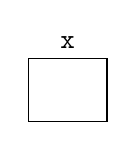
\begin{tikzpicture}
\node[draw,rectangle,minimum width=10mm,minimum height=8mm] at (0,0) {};
\node at (0,6mm) {\texttt{x}};
\end{tikzpicture}
\caption{容器}
\label{basic:cpp:fig:variable}
\end{figure}

\paragraph{}變數的用途就是為了把數字裝到變數中,
\begin{code}[h!]
\centering
\begin{tabular}{c}
\begin{lstlisting}
#include <iostream>
using namespace std;
int main() {
  int x;             // 宣告變數 x
  x = 5;             // 把整數 5 裝進 x 裡面
  cout << x << endl; // 印出變數 x 存的值
}
\end{lstlisting}
\end{tabular}
\caption{變數的用途}
\label{basic:cpp:code:use:variable}
\end{code}

\paragraph{}宣告變數的種類除了\lstinline!int! (即整數) 之外,還有其他不同的種類,以後會慢慢介紹。此外,程式碼 \ref{basic:cpp:code:use:variable} 中 \lstinline!x = 5;! 這行\textbf{不要}和數學中的「等於」搞混。
  
\paragraph{}練習看看,若把上個投影片「\lstinline!x = 5;!」改成以下狀況,會出現什麼事?該怎麼解釋這些現象呢?
\begin{itemize}
\item \lstinline!x = 5.0;!
\item \lstinline!x = 0.5;!
\item \lstinline!5 = x;!
\end{itemize}

\paragraph{}這些練習目的是要讓你\textbf{真正了解}問題出現時的現象,了解出問題的原因才有辦法 debug,為什麼會出現這些現象我們繼續下去就知道了。

\paragraph{多變數宣告}宣告兩個整數可以寫成這樣:
\begin{code}[h!]
\centering
\begin{tabular}{c}
\begin{lstlisting}
int a;
int b;
\end{lstlisting}
\end{tabular}
\caption{宣告兩個變數}
\label{basic:cpp:code:two:declare}
\end{code}

\paragraph{}兩個變數更可以簡化成這樣:
\begin{code}[h!]
\centering
\begin{tabular}{c}
\begin{lstlisting}
int a, b;
\end{lstlisting}
\end{tabular}
\caption{宣告兩個變數,簡化版}
\label{basic:cpp:code:two:declare:abbr}
\end{code}

\paragraph{}以此類推,宣告三個整數也是如法炮製,如程式碼 \ref{basic:cpp:code:three:declare:abbr}:
\begin{code}[h!]
\centering
\begin{tabular}{c}
\begin{lstlisting}
int a, b, c;
\end{lstlisting}
\end{tabular}
\caption{宣告三個變數}
\label{basic:cpp:code:three:declare:abbr}
\end{code}

\paragraph{變數初始化}剛剛我們說過變數個作用就是\textbf{裝東西},那如果容器不塞東西會發生什麼事呢?比如程式碼 \ref{basic:cpp:code:non:init}。

\begin{code}[h!]
\centering
\begin{tabular}{c}
\begin{lstlisting}
  #include <iostream>
  using namespace std;
  int main() {
    int x;             // 宣告變數 x
    cout << x << endl; // 印出變數 x 存的值
  }
\end{lstlisting}
\end{tabular}
\caption{變數不初始化,會發生什麼事呢?}
\label{basic:cpp:code:non:init}
\end{code}

\paragraph{}程式碼 \ref{basic:cpp:code:non:init} 可以多試幾次,一般來說,\texttt{C++} 中,所有變數都要自己去\textbf{初始化}。例如:\lstinline!x = 5;!,把整數 5 丟給 \lstinline!x! 等等。因為沒有初始化過的變數,裡面裝的資料是\textbf{不確定}的。

\paragraph{}或許你很幸運看到 \lstinline!x! 都是 \lstinline!0!,但那只是\textbf{恰巧}而已,因此有時候程式有 bug 時,不妨檢查一下是否存在這個原因。

\begin{figure}[h!]
\centering
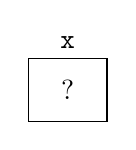
\begin{tikzpicture}
\node[draw,rectangle,minimum width=10mm,minimum height=8mm] at (0,0) {$?$};
\node at (0,6mm) {\texttt{x}};
\end{tikzpicture}
\caption{沒有被初始化的變數}
\label{basic:cpp:fig:non:init:variable}
\end{figure}

\paragraph{}要解決變數沒有初始化的問題,有兩個常用的方法,原則上都是\index{賦值}{\textbf{賦值}},方法會在稍後提到。

\subsubsection{輸入}

\paragraph{}執行以下程式會發生什麼事呢?

\begin{code}[h!]
\centering
\begin{tabular}{c}
\begin{lstlisting}
#include <iostream>
using namespace std;
int main() {
  int x;
  cin >> x;
  cout << x << endl;
}
\end{lstlisting}
\end{tabular}
\caption{輸入}
\label{basic:cpp:code:cin}
\end{code}

\paragraph{}大家可以試著執行看程式碼 \ref{basic:cpp:code:cin},如果沒發生什麼事,試著輸入「\lstinline!1!」再按 enter 鍵,會發生什麼事呢?
\paragraph{}和輸出相對,「\lstinline!cin!」代表輸入符號,可以輸入後面變數的資料。輸入的資料和我們宣告變數的\index{型態}{\textbf{型態}}有關,在此例中,\lstinline!x! 是整數,因此可以\textbf{輸入一個整數}。
\paragraph{}\textbf{注意}! \lstinline!cin! 的 \textbf{\lstinline!>>!} 不要和 \lstinline!cout! 的 \textbf{\lstinline!<<!} 搞混。以下練習讀者們可以試試看會發生什麼事,重點在\textbf{觀察產生的現象}:

\begin{itemize}
\item 輸入「\texttt{5.0}」再按 enter 鍵呢?
\item 輸入「\texttt{0.5}」再按 enter 鍵呢?
\item 輸入「\texttt{XD}」再按 enter 鍵呢?
\end{itemize}

\paragraph{多變數輸入}\index{輸入!多變數輸入}{多變數輸入}和輸出類似:

\begin{code}[h!]
\centering
\begin{tabular}{c}
\begin{lstlisting}
int x, y;
cin >> x >> y;
\end{lstlisting}
\end{tabular}
\caption{輸入多變數}
\label{basic:cpp:code:cin:variables}
\end{code}

\paragraph{}唯一要注意的一點是,有些題目會要我們輸入「換行」相隔的數,我們不需要在輸入中加入「\lstinline!endl!」,否則程式容易出錯。

\subsubsection{資料型態}

\paragraph{}既然有裝整數的容器,那麼當然也可以宣告裝「小數點」的容器啦!這些不同用途的容器我們稱為「\index{資料型態}{\textbf{資料型態}}」。表 \ref{basic:cpp:table:primitive:type} 代表 \texttt{C++} 常用的資料型態,詳細內容之後再介紹,先來用看看這些東西。

\begin{table}[h!]
\centering
\begin{tabular}{|c|c|c|}
\hline
關鍵字 & 意義 & 備註\\
\hline
\hline
\index{資料型態!布林值}{\lstinline!bool!} & 布林值 & 只有 \lstinline!true! 和 \lstinline!false!\\
\hline
\lstinline!int! & 整數 &\\
\hline
\lstinline!long long! & 長整數 & 存比較大的整數,以後會介紹\\
\hline
\lstinline!double!    & \textbf{浮點數} & 也就是小數點\\
\hline
\end{tabular}
\caption{資料型態}
\label{basic:cpp:table:primitive:type}
\end{table}

\paragraph{布林值}\index{布林值}{布林值}是一種資料型態,只來裝兩種數值:「\lstinline!true!」和「\lstinline!false!」,宣告方法和 \lstinline!int! 類似,如程式碼 \ref{basic:cpp:code:declare:bool}:

\begin{code}[h!]
\centering
\begin{tabular}{c}
\begin{lstlisting}
bool b;
\end{lstlisting}
\end{tabular}
\caption{布林值宣告}
\label{basic:cpp:code:declare:bool}
\end{code}

\paragraph{}值得注意的是,兩個不同資料型態不能同時宣告在同一行,如程式碼 \ref{basic:cpp:code:forbidden:comma}。其實在 \texttt{C++} 當中,\index{逗號運算子}{逗號}有\textbf{特殊意義},不要想成一般的「逗號」。

\begin{code}[h!]
\centering
\begin{tabular}{c}
\begin{lstlisting}
int a, bool b;
\end{lstlisting}
\end{tabular}
\caption{不同的宣告不能用「逗號」隔開}
\label{basic:cpp:code:forbidden:comma}
\end{code}

\paragraph{賦值}將一個「數值」裝進一個變數中,稱為\textbf{賦值}。例如,程式碼 \ref{basic:cpp:code:assignment} 把整數 5 裝進整數變數 \lstinline!x! 中:

\begin{code}[h!]
\centering
\begin{tabular}{c}
\begin{lstlisting}
int x;
x = 5;
\end{lstlisting}
\end{tabular}
\caption{賦值}
\label{basic:cpp:code:assignment}
\end{code}

\paragraph{}當然,我們每次如果一行宣告,一行賦值也太麻煩,因此有簡化的寫法,變數宣告和賦值可以寫在一起:

\begin{code}[h!]
\centering
\begin{tabular}{c}
\begin{lstlisting}
int x = 5;
\end{lstlisting}
\end{tabular}
\caption{賦值簡化}
\label{basic:cpp:code:assignment:simple}
\end{code}

\paragraph{練習}下面有一段程式碼:

\begin{code}[h!]
\centering
\begin{tabular}{c}
\begin{lstlisting}
bool b;
cout << b << endl;
\end{lstlisting}
\end{tabular}
\label{basic:cpp:code:practice:bool}
\end{code}

\paragraph{}對程式碼的 \lstinline!b! 做以下賦值,會發生什麼事?
\begin{itemize}
\item \lstinline!b = true;!
\item \lstinline!b = false;!
\item \lstinline!b = 2;!
\item \lstinline!b = 0;!
\item \lstinline!b = -1;!
\end{itemize}
  
\paragraph{布林值的重要觀念}\texttt{C++} 中,「\textbf{非零整數}」會被當做「\lstinline!true!」,印出時也會印出一個非零整數 (\textbf{通常是 1})。「0」會被當做「\lstinline!false!」,印出時會印出「\textbf{0}」。
\paragraph{}這個特性在之後會\textbf{非常}常用!大家要注意!

\paragraph{浮點數}先跳過 \lstinline!long long!,先知道 \lstinline!long long! 也是存整數就好。(謎之音:「那幹嘛現在說= =」)這裡先來講一下浮點數,浮點數也就是存\textbf{小數點}的資料型態,宣告方法如下:

\begin{code}[h!]
\centering
\begin{tabular}{c}
\begin{lstlisting}
double d;
\end{lstlisting}
\end{tabular}
\caption{浮點數宣告}
\label{basic:cpp:code:declare:double}
\end{code}

\paragraph{}賦值和前面都一樣,不同的是浮點數有一些特別的表示法:
\begin{itemize}
\item 如果要把 \lstinline!1.0! \lstinline!d! $\Rightarrow$ \lstinline!d = 1.0;!,這是最基本的賦值
\item 稍微有變化一點,如果是 \lstinline!0.5! 的話,可以簡化為 \lstinline!.5! $\Rightarrow$ \lstinline!d = .5;!
\item 接著是\index{科學記號}{\textbf{科學記號}}
  \begin{itemize}
  \item \lstinline!18.23e5! 代表 $18.23\times{10^5}$
  \item \lstinline!5.14e-6! 代表 $5.14\times{10^{-6}}$
  \end{itemize}
\end{itemize}

\subsection{算術運算子}
\subsubsection{運算性質}

\paragraph{}算術運算子有以下五個:
\begin{table}[h!]
\centering
\begin{tabular}{|c|c|c|c|}
\hline
算術運算子      & 意義 & 運算順序 & 結合性\\
\hline
\hline
\lstinline!+! & 加法 & 6 & 左$\rightarrow$右\\
\hline
\lstinline!-! & 減法 & 6 & 左$\rightarrow$右\\
\hline
\lstinline!*! & 乘法 & 5 & 左$\rightarrow$右\\
\hline
\lstinline!/! & 除法 & 5 & 左$\rightarrow$右\\
\hline
\lstinline!%! & 取餘數 & 5 & 左$\rightarrow$右\\
\hline
\end{tabular}
\caption{算術運算子}
\label{basic:cpp:table:operator:arithmetic}
\end{table}

\paragraph{}如果不管\textbf{運算順序}和\textbf{結合性},一般來說可以用五則運算來理解,只不過程式跟數學還是有差距,舉個例子:$1+2+3$ 會是多少?

\paragraph{}這個問題很顯然答案會是 $6$,但是程式為什麼會計算出答案呢?我們先建立起\index{二元運算}{\textbf{二元運算}}的觀念:

\begin{mydef}
\index{二元運算}{\textbf{二元運算}}由一個\index{二元運算!運算子}{\textbf{運算子}}和兩個\index{二元運算!運算元}{\textbf{運算元}}構成,例如:$1+2$:「$+$」稱為「運算子」,「$1$」和「$2$」稱為運算元 (我們常稱為「被加數」和「加數」)。
\label{basic:cpp:def:binary:operator}
\end{mydef}

\subsubsection{結合性與運算順序}

\paragraph{}我們可以知道「加減乘除餘」都是二元運算,因此,我們回到原來的問題:$1+2+3$ 到底是先算 $1+2$、還是先算 $2+3$ 呢?

\paragraph{}這時我們就會出現大麻煩了!儘管在這裡先算後算是沒有太大的問題,但是在 $1-2-3$ 的情況下,先算 $1-2$、還是 $2-3$ 這個問題就變成此時需要解決的問題。

\paragraph{}計算機普遍採用的解法就是「決定運算的\textbf{方向}」。例如:
\begin{itemize}
\item 先算 $1+2=3$,再算 $\textbf{3}+3=6$
\item 先算 $2+3=5$,再算 $1+\textbf{5}=6$
\end{itemize}

\paragraph{}決定運算方向對「計算機」而言\textbf{意義重大}!同樣的想法可套進剛剛的 $1-2-3$ 中:

\begin{itemize}
\item 我們直觀上會先算 $1-2=-1$,再算 $-1-3=-4$。
\item 因此 \texttt{C++} 在設計上也會把加減乘除餘的\index{二元運算!結合性}{\textbf{結合性}}「設定」成\textbf{從左到右算}。
\end{itemize}

\paragraph{}我們回頭看表 \ref{basic:cpp:table:operator:arithmetic},可以看出在結合性那一欄定義了每個運算子的運算順序。

\paragraph{}接著我們處理更複雜的問題--四則運算:$1+2*3-4$。同樣地,我們的運算規則是「\textbf{先乘除餘,後加減}」,因此 \texttt{C++} 發展出一套類似的規則,稱做\index{二元運算!運算順序}{\textbf{運算順序}}。

\begin{itemize}
\item 運算順序小的優先運算,在表 \ref{basic:cpp:table:operator:arithmetic} 中 \texttt{C++} 定義了每個運算子的\textbf{優先權}
\item 若運算順序相同,則依照運算方向做計算。
\end{itemize}

\paragraph{}因此我們知道整個運算式的運算順序如下:

\begin{align*}
  & 1+\textbf{2*3}-4 &*\text{ 的運算順序最高}\\
= & \textbf{1+6}-4   &\text{加法和減法運算順序相同,依照結合性從左到右算}\\
= & \textbf{7-4}     &\text{依照結合性從左到右算}\\
= & 3
\end{align*}

\paragraph{}\texttt{C++} 的四則運算用\textbf{優先順序}和\textbf{結合性}來處理,這件事情非常重要,稍後就會知道為什麼。

\subsubsection{整數除法與除零問題}

\paragraph{整數除法}以下程式碼可能會讓你感到驚奇:
\begin{itemize}
\item \lstinline!cout << 8 / 5 << endl;! 的結果?{\textbf{Ans: 1}}
\item \lstinline!cout << 8.0 / 5.0 << endl;! 的結果?{\textbf{Ans: 1.6}}
\end{itemize}

\paragraph{}其原因出在於,在 \lstinline!8 / 5! 中,\lstinline!8! 和 \lstinline!5! 被視為 \lstinline!int!,因此 \texttt{C++} 會做「\index{整數除法}{\textbf{整數除法}}」;而在 \lstinline!8.0 / 5.0! 中,\lstinline!8.0! 和 \lstinline!5.0! 被視為浮點數 \lstinline!double!,因此會做「\index{浮點數除法}{\textbf{浮點數除法}}」。

\paragraph{除以零}除法還有另外一個問題點,那就是\index{除零問題}{\textbf{除以零}},我們知道數學上是不能除以零的,那程式呢?下面的狀況讀者們也請多做嘗試,看看會發生什麼結果。

\begin{itemize}
\item \lstinline!cout << 1 / 0 << endl;!
\item \lstinline!cout << 0 / 0 << endl;!
\item \lstinline!cout << 1.0 / 0.0 << endl;!
\item \lstinline!cout << 0.0 / 0.0 << endl;!
\end{itemize}

\paragraph{}\textbf{註}:有些 IDE 如 Visual C++ 會直接擋住除以零,不讓你編譯,如果無法編譯成功,那麼就嘗試「繞過」他,例如:宣告一個變數,把分母裝 \lstinline!0! 進去再試試看。
\paragraph{}\textbf{注意}:通常上面的程式碼在編譯時可以過,但是在執行時會出些狀況,各位知道出了哪些狀況就好,不用了解太詳細。

\subsubsection{應用:取餘數}

\paragraph{}\texttt{C++} 的 \lstinline!%! 運算子會有跟我們想像中不太一樣的現象,首先我們可以觀察一下 \texttt{C++} 怎麼做的:
\begin{itemize}
\item \lstinline!cout << 5 % 3 << endl;! 會輸出什麼?{\textbf{Ans:2}}
\item \lstinline!cout << (-5) % 3 << endl;! 呢?{\textbf{Ans:-2}}
\end{itemize}

\paragraph{}大部分的人會認為,\lstinline!%! 就是「取餘數」,但事實上並不完全是這樣子,如果在下面 \lstinline!-2! 的例子,應該結果是要 \lstinline!1! 才對,這也是 \texttt{C++} 一個\textbf{奇怪的特性}。

\paragraph{}解決方法?要怎麼做出取餘數的效果呢?以下提供一個解法:
  
\begin{enumerate}
\item 假設 \lstinline!n! 要 mod \lstinline!m! ...
\item 首先,我們取 \lstinline!n % m!
  \begin{itemize}
  \item 如果 $n\geq{0}${,會得到介於 $0$ 到 $m-1$ 的數字}
  \item 如果 $n<0${,會得到介於 $-(m-1)$ 到 $0$ 的數字}
  \end{itemize}
\item 接著加上 \lstinline!m!,變成 \lstinline!n % m + m!
  \begin{itemize}
  \item 如果 $n\geq{0}${,會得到介於 $m$ 到 $2m-1$ 的數字}
  \item 如果 $n<0${,會得到介於 $-(m-1)+m=1$ 到 $m$ 的數字}
  \item 全都修成正值了!{\textbf{但還差最後一步 ...}}
  \end{itemize}
\item 最後,再 mod \lstinline!m! 一次,把所有數字修正回 $0$ 到 $m-1$ 之間。
  \begin{itemize}
  \item 大功告成啦! \lstinline!(n % m + m) % m!
  \end{itemize}
\end{enumerate}

\subsubsection*{練習題}
\begin{itemize}
\item \label{basic:cpp:problem:uva:10071}\href{http://pcshic.github.io/uniDog/problem/p10071/}{UVa 10071 - Back to High School Physics}\\這題只要能夠讀懂題意就不難寫。如果不知道怎樣讀取多筆測資請先參考迴圈部分 (EOF 版)。
\item \label{basic:cpp:problem:uva:10300}\href{http://pcshic.github.io/uniDog/problem/p10300/}{UVa 10300 - Ecological Premium}\\一樣能讀懂題意就不難寫。
\end{itemize}

\subsection{比較和邏輯運算子}
\subsubsection{比較運算子}

\paragraph{}比較運算子如表 \ref{basic:cpp:table:operator:comparison}:
\begin{table}[h!]
\centering
\begin{tabular}{|c|c|c|c|}
\hline
比較運算子 & 意義 & 運算順序 & 結合性\\
\hline
\hline
\lstinline!==! & 等於 & 9 & 左$\rightarrow$右\\
\hline
\lstinline"!=" & 不等於 & 9 & 左$\rightarrow$右\\
\hline
\lstinline!>!  & 大於 & 8 & 左$\rightarrow$右\\
\hline
\lstinline!<!  & 小於 & 8 & 左$\rightarrow$右\\
\hline
\lstinline!>=! & 不小於 & 8 & 左$\rightarrow$右\\
\hline
\lstinline!<=! & 不大於 & 8 & 左$\rightarrow$右\\
\hline
\end{tabular}
\caption{比較運算子}
\label{basic:cpp:table:operator:comparison}
\end{table}

\paragraph{}和數學的大於小於概念類似,只是要\textbf{注意}!\texttt{C++} 的等於寫作「\lstinline!==!」,不要和賦值的「\lstinline!=!」搞混。
\paragraph{回傳值} \texttt{C++} 程式當中有\index{回傳值}{回傳值}的概念,舉例來說:\lstinline!cout << (3 < 5) << endl;! 這一行會發生什麼事呢?要解釋這一段程式有點複雜,我們慢慢講起。
\paragraph{}比較運算子也算是一種\textbf{二元運算},他會比較兩邊數字大小,如果是正確的,則為 \lstinline!true!、否則就是 \lstinline!false!。這種概念我們稱為「\textbf{回傳值}」。
\paragraph{}回傳值也會有資料型態,由此可見比較運算子的回傳值是布林值 \lstinline!bool!,例如 \textbf{\lstinline!3 < 5!} 的回傳值就是 \lstinline!true!。
\paragraph{}但是還沒完,因為我們發現剛剛那一行程式碼不是印出 \lstinline!true!,怎麼回事呢?根據 \texttt{C++} 的規則,\lstinline!true! 通常會當作\textbf{非零},因此會印出一個非零的數字 (通常是 \lstinline!1!);反之,如果是 \lstinline!false!,就會當作是 \lstinline!0!。以此出發,這會延伸到之後有很多技巧。

\paragraph{運算簡化}例如,判斷\textbf{不}整除直觀來想就是「檢查 \lstinline!n! 取 \lstinline!m! 的餘數是否非零」,我們利用前面學到的比較運算子和算術運算子可以得出 \lstinline"n % m != 0"。

\paragraph{}但是這一個判斷還可以進一步簡化,如果 \lstinline!n % m! 結果不是零,如果在條件判斷時會被當作 \lstinline!true!,否則就被當作 \lstinline!false!,因此很多時候就只要簡寫成 \lstinline!n % m! 就可以了。

\begin{table}[h!]
\centering
\begin{tabular}{|c|c|c|}
\hline
& \lstinline"n % m != 0" & \lstinline!n % m!\\
\hline\hline
當 \lstinline!n % m! 不為零 & \lstinline!true! & \lstinline!true!\\
\hline
當 \lstinline!n % m! 為零 & \lstinline!false! & \lstinline!false!\\
\hline
\end{tabular}
\caption{真值表}
\label{basic:cpp:table:practice:truth}
\end{table}

\paragraph{}簡化的寫法大多時候可以取代原來一般寫法,且通常比較運算子要和 \lstinline!if!、\lstinline!else! 配合,之後會介紹這兩個東西。

\subsubsection{邏輯運算子}

\paragraph{}\index{邏輯運算子}{邏輯運算子}有以下三個:
\begin{table}[h!]
\centering
\begin{tabular}{|c|c|c|c|}
\hline
邏輯運算子 & 意義 & 運算順序 & 結合性\\
\hline
\hline
\lstinline!&&! & 且 & 13 & 左$\rightarrow$右\\
\hline
\lstinline!||! & 或 & 14 & 左$\rightarrow$右\\
\hline
\lstinline"!"  & 非 & 3  & \textbf{右$\rightarrow$左}\\
\hline
\end{tabular}
\caption{邏輯運算子}
\label{basic:cpp:table:operator:logical}
\end{table}

\paragraph{}邏輯運算子一般來說是連接比較運算子,例如:\lstinline!1 < x && x < 5!。

\paragraph{}舉個大家容易誤解的例子,如果要判斷 \lstinline!x! 是否介於 \lstinline!a! 和 \lstinline!b! 之間能不能寫成 \lstinline!a <= x <= b;! 呢?答案是{\color{red}不行}。乍看之下似乎符合數學運算式,但是讀者必須注意,這裡是 \texttt{C++},因此我們需要用 \texttt{C++} 的觀念去切入這個問題。
\paragraph{}我們可以採用回傳值的觀點,從表 \ref{basic:cpp:table:operator:logical} 可以知道,\lstinline!<=! 運算子在列出很多個時,會\textbf{由左到右算},因此在左側的 \textbf{\lstinline!a <= x!} 會先算出 \lstinline!true! 或者是 \lstinline!false!。
\paragraph{}假設 \lstinline!a=-4!、\lstinline!b=-1!、\lstinline!x=-2!,我們\textbf{預期}結果是 \lstinline!true!,接著分析 \texttt{C++} 會怎麼處理 \lstinline!a <= x <= b!。
\begin{itemize}
\item \texttt{C++} 會先計算 \lstinline!a <= x! 得到 \lstinline!true!
\item 接著計算 \lstinline!true <= b!
\item 我們知道 \lstinline!true! 通常是 \lstinline!1!
\item \lstinline!a <= x <= b! 的回傳值就會是 \lstinline!false!
\end{itemize}

\paragraph{}反過來,\lstinline!a <= x! 是 \lstinline!false! 的狀況也會有同樣的問題。
\paragraph{}如果我們要解決此狀況,那麼就勢必要用邏輯運算子:\lstinline!a <= x && x <= b!。這個觀念常常是剛上手 \texttt{C++} 的人常常踩到的誤區,可以多注意。

\paragraph{}我們先前是對「判斷不整除」進行簡化,那我們要怎麼簡化「判斷整除」呢? \lstinline!n % m == 0! 可以用「\lstinline"!" 運算子」變成 \lstinline"!(n % m != 0)",接著使用剛剛的簡化規則,最後變成 \lstinline"!(n % m)"。

\subsubsection{短路運算}

\paragraph{}\texttt{C++} 的邏輯運算屬於「\index{邏輯運算子!短路運算}{\textbf{短路運算}}」,當我們在計算一個判斷式時,如果我們已經可以確認其結果,之後的判斷就\textbf{不會再進行}。以下講述 \lstinline!&&! 運算子和 \lstinline!||! 運算子的行為:

\begin{itemize}
\item \lstinline!A && B!:實際上當 \lstinline!A! 是 \lstinline!false!,也就是確定整個運算式\textbf{必為} \lstinline!false!,則程式會\textbf{跳過} \lstinline!B!,下面程式碼可以試試看:

\begin{code}[h!]
\centering
\begin{tabular}{c}
\begin{lstlisting}
int i, j;
i = j = 0;
if ((i++ < 0) && (j++ > 0))
  cout << "XD" << endl; // 這行不會輸出
cout << i << " " << j << endl; // i 為 1,j 為 0
\end{lstlisting}
\end{tabular}
\caption{範例}
\label{basic:cpp:code:short:cut}
\end{code}

\item \lstinline!A || B!:只要 \lstinline!A! 是 \lstinline!true!,也就是確定整個運算式\textbf{必為} \lstinline!true!,則程式會\textbf{跳過} \lstinline!B!

\begin{code}[h!]
\centering
\begin{tabular}{c}
\begin{lstlisting}
int i, j;
i = j = 0;
if ((i++ >= 0) || (j++ < 0))
  cout << "XD" << endl; // 會輸出 XD
cout << i << " " << j << endl; // i 為 1,j 為 0
\end{lstlisting}
\end{tabular}
\caption{範例}
\label{basic:cpp:code:short:cut:2}
\end{code}

\end{itemize}

\subsubsection*{練習題}
\begin{itemize}
\item \label{basic:cpp:problem:uva:10055}\href{http://pcshic.github.io/uniDog/problem/p10055/}{UVa 10055 - Hashmat the brave warrior}\\%
取絕對值有兩種做法,一種是用 \lstinline!if! 判斷;另一種是呼叫函數 \lstinline!abs()! 就好了。\lstinline!abs()! 函數被定義在 \lstinline!<cstdlib>! 中,雖然沒有 \lstinline!include! 在 Visual C++ 依然能編譯過,但是上傳時因為編譯器的原因會導致\index{編譯錯誤}{\textbf{編譯錯誤}} (Compilation Error, CE)。\\%
另外要注意這一題的整數型態需用 \lstinline!long long!,用 \lstinline!int! 會造成「\index{溢位現象}{溢位現象}」,這個原因會在後面說明。
\item \label{basic:cpp:problem:uva:11172}\href{http://pcshic.github.io/uniDog/problem/p11172/}{UVa 11172 - Relational Operators}\\%
能夠理解題意就不難解決此道問題。
\item \label{basic:cpp:problem:uva:11942}\href{http://pcshic.github.io/uniDog/problem/p11942/}{UVa 11942 - Lumberjack Sequencing}\\%
依序給你一些鬍子的長度,問你這些鬍子是不是由長到短,或是由短到長排列。
\end{itemize}

\subsection{位元運算子}
\subsubsection{\lstinline!int! 和 \lstinline!long long! 的儲存形式}

\paragraph{}在此節我們要講\index{位元運算子}{位元運算子},但在一開始我們要先了解 \lstinline!int! 在電腦當中怎麼儲存的,因此要先介紹一些觀念。

\begin{itemize}
\item \index{位元}{\textbf{位元}} (bit, b):計算機儲存資料的基本單位,只儲存 \textbf{0 和 1}
\item \index{位元組}{\textbf{位元組}} (byte, B):因為位元很多,所以我們習慣上把 8 個位元「打包起來」,變成一個位元組

\begin{table}[h]
\centering
\begin{tabular}{|c|}
\hline
01001010\\
\hline
\end{tabular}
\caption{位元組}
\label{basic:cpp:table:byte}
\end{table}

\item 常見應用
  \begin{itemize}
  \item KB、MB、GB、TB、PB:資料大小
  \item Kbps、Mbps、Gbps:資料傳輸速度
  \end{itemize}
\end{itemize}

\paragraph{}以 \lstinline!int! 來說,他至少使用 \textbf{2 個位元組}來紀錄資料,有些讀者可能會有疑問說:「不是都 4 個位元組嘛?」其實當初定義時,\lstinline!int! 只有\textbf{定義}成「至少」2 個位元組,只是現在的電腦大多是 4 個位元組。

\begin{table}[h!]
\centering
\begin{tabular}{|c|c|}
\hline
型態 & 長度\\
\hline
\hline
\lstinline!bool!      & 1 位元組\\
\hline
\lstinline!int!       & 2 或 \textbf{4} 位元組\\
\hline
\lstinline!long long! & 4 或 \textbf{8} 位元組\\
\hline
\lstinline!double!    & 8 位元組\\
\hline
\end{tabular}
\caption{位元組長度}
\label{basic:cpp:table:byte:length}
\end{table}

\paragraph{}表 \ref{basic:cpp:table:byte:length} 標示每個資料型態使用多少位元組來紀錄資料,在 \lstinline!int! 和 \lstinline!long long! 部分,用粗體來表示現在大部分的機器所使用的位元組數。以下討論就使用 \lstinline!int! 為 4 個位元組、\lstinline!long long! 為 8 個位元組,不再贅述。

\paragraph{\lstinline!int! 表示法}一般來說,\lstinline!int! 由 4 個位元組組成

\begin{table}[h!]
\centering
\begin{tabular}{|c|c|c|c|}
\hline
10100010 & 00110011 & 00100111 & 10101101\\
\hline
\end{tabular}
\caption{\lstinline!int! 的位元組}
\label{basic:cpp:table:int}
\end{table}

\paragraph{}可以視為一個長度是 32 的二進位數字,我們將位數依照高低編號,如表 \ref{basic:cpp:table:int:variables},$x_{31}$ 表示正負號,若 $x_{31}$ 為 \lstinline!0! 代表此 \lstinline!int! 是正數,反之則為負數。

\begin{table}[h!]
\centering
\begin{tabular}{|c|c|c|c|}
\hline
$x_{31}x_{30}\cdots{x_{24}}$ & $x_{23}x_{22}\cdots{x_{16}}$ & $x_{15}x_{14}\cdots{x_{8}}$ & $x_{7}x_{6}\cdots{x_{0}}$\\
\hline
\end{tabular}
\caption{二進位 \lstinline!int!}
\label{basic:cpp:table:int:variables}
\end{table}

\paragraph{}因為 \lstinline!int! 的儲存方式很特別,要多花一些力氣說明。

\paragraph{\lstinline!int! 存正數的情況}當 \lstinline!int! 儲存正數時,是依照一般二進位方式儲存。例如 \lstinline!int x = 1;!

\begin{table}[h!]
\centering
\begin{tabular}{|c|c|c|c|}
\hline
{\color{red}0}0000000 & 00000000 & 00000000 & 0000000{\color{red}1}\\
\hline
\end{tabular}
\caption{\lstinline!1! 的二進位表示法}
\label{basic:cpp:table:binary:1}
\end{table}

\paragraph{}當 \lstinline!int x = 255;! 時如表 \ref{basic:cpp:table:binary:255}。

\begin{table}[h!]
\centering
\begin{tabular}{|c|c|c|c|}
\hline
{\color{red}0}0000000 & 00000000 & 00000000 & {\color{red}11111111}\\
\hline
\end{tabular}
\caption{\lstinline!255! 的二進位表示法}
\label{basic:cpp:table:binary:255}
\end{table}

\paragraph{\lstinline!int! 存負數的情況}上面情況都不難,比較有意思的是當它存負數時,怎麼表示呢?例如下面的 \lstinline!int x = -1;!:

\begin{table}[h!]
\centering
\begin{tabular}{|c|c|c|c|}
\hline
\textbf{1}1111111 & 11111111 & 11111111 & 11111111\\
\hline
\end{tabular}
\caption{存 \lstinline!-1! 的情況}
\label{basic:cpp:table:int:-1}
\end{table}

\paragraph{}要理解負數的儲存方法 (謎之音:「根本黑魔法!」),我們嘗試看看 \lstinline!(-1)+1!,我們知道 $(-1)+1=0$,那麼以這種表示法相加的結果是:

\begin{table}[h!]
\centering
\begin{tabular}{|c|r|c|c|c|}
\hline
 & 11111111 & 11111111 & 11111111 & 11111111\\
\hline
\lstinline!+! & 00000000 & 00000000 & 00000000 & 00000001\\
\hline
\hline
 & {\color{red}1}00000000 & 00000000 & 00000000 & 00000000\\
\hline
\end{tabular}
\end{table}

\paragraph{}紅色的 {\color{red}1} 因為超過 32 位元,所以被捨棄,稱為\index{溢位}{\textbf{溢位}}。
\paragraph{}這種表示法稱為\textbf{二補數 (2's complement)},好處是減法和加法只需要用溢位的方式就可以處理掉,這在底層硬體實作上帶來許多方便,缺點當然是不好理解負數的儲存方法。要想像負數 \lstinline!-x! 的表示法,訣竅是 \lstinline!(-x)+x! 會因為溢位而等於 \lstinline!0!。
\paragraph{}大致上來說,最特別的兩個數,一個是 \lstinline!0!,在此表示法中會是\textbf{全 0};而 \lstinline!-1! 會是\textbf{全 1},這兩個數字在很多時候會很好用,可以稍微記得這個結論。
\paragraph{}以下練習看看:

\begin{itemize}
\item \lstinline!int x = -2;!
\item \lstinline!int x = -256;!
\end{itemize}
  
\subsubsection{位元運算子}

\paragraph{}位元運算子是大家比較難理解的運算子,但是在效能優化上,或是在一些特殊的題目時是很有用的,以下分別講述這些運算子的功用與概念。
\begin{table}[h!]
\centering
\begin{tabular}{|c|c|c|c|}
\hline
位元運算子 & 意義 & 運算順序 & 結合性\\
\hline
\hline
\lstinline!<<! & 左移運算子 & 7 & 左$\rightarrow$右\\
\hline
\lstinline!>>! & 右移運算子 & 7 & 左$\rightarrow$右\\
\hline
\lstinline!&!  & 位元 \texttt{and} & 10 & 左$\rightarrow$右\\
\hline
\lstinline!^!  & 位元 \texttt{xor} & 11 & 左$\rightarrow$右\\
\hline
\lstinline!|!  & 位元 \texttt{or} & 12 & 左$\rightarrow$右\\
\hline
\lstinline!~!  & 1's 補數  & 3 & \textbf{右$\rightarrow$左}\\
\hline
\end{tabular}
\caption{位元運算子}
\label{basic:cpp:table:operator:bitwise}
\end{table}

\paragraph{左移和右移運算子}左移運算子和右移運算子代表在位元操作上左移和右移 k 個位元,但注意不要和 \lstinline!cin! 與 \lstinline!cout! 的 \lstinline!<<!、\lstinline!>>! 混淆。

\paragraph{}舉例來說,\lstinline!2 << 2!{ $\Rightarrow$ \lstinline!8!} 即是把 2 在二進位的位元往左移 2 格:

\begin{table}[h!]
\centering
\begin{tabular}{|c|c|c|c|}
\hline
00000000 & 00000000 & 00000000 & 000000{\color{red}10}\\
\hline
\end{tabular}
\begin{center}$\Downarrow$\end{center}
\begin{tabular}{|c|c|c|c|}
\hline
00000000 & 00000000 & 00000000 & 0000{\color{red}10}00\\
\hline
\end{tabular}
\caption{左移的情況}
\label{basic:cpp:table:left:shift}
\end{table}

\paragraph{}類似的情況,\lstinline!5 >> 1!{ $\Rightarrow$ \lstinline!2!} 把 5 在二進位的位元往右移一格,最右邊多餘的 \lstinline!1! 會被捨棄:

\begin{table}[h!]
\centering
\begin{tabular}{|c|c|c|c|}
\hline
00000000 & 00000000 & 00000000 & 00000{\color{red}101}\\
\hline
\end{tabular}
\begin{center}$\Downarrow$\end{center}
\begin{tabular}{|c|c|c|c|}
\hline
00000000 & 00000000 & 00000000 & 000000{\color{red}10}\\
\hline
\end{tabular}
\caption{右移的情況}
\label{basic:cpp:table:right:shift}
\end{table}

\paragraph{}不管是左移還是右移,移出去的位元會被捨棄,這也是\index{溢位}{溢位}的一種,但在左移右移會影響到 $x_{31}$ 時會比較複雜,因為我們知道 $x_{31}$ 決定正負號,以下例子讀者們可以試試看,應該會出乎意料之外:
\begin{itemize}
\item \lstinline!2147483647 << 1!
\item \lstinline!-5 >> 1!
\item \lstinline!(2147483647 << 1) >> 1!
\end{itemize}

\paragraph{}那左移和右移運算子有什麼應用呢?我們觀察一下 \lstinline!a << k! 會得到什麼數字呢? 那 \lstinline!a >> k! 呢?

\paragraph{}一般來說 \lstinline!a << k! 會得到 $a\times{2^k}$,\lstinline!a >> k! 會得到 $a / 2^k$,有些情況比較複雜,大家看看就好,起碼對這些運算「有感覺」。

\paragraph{\texttt{and}、\texttt{xor}、\texttt{or} 運算子}
    對於兩個位元 \lstinline!x! 和 \lstinline!y!,遵守以下運算規則:


\begin{table}[h!]
\centering
\caption{三種運算子}
\label{basic:cpp:table:operator:bitwise:2}
\begin{subtable}{.23\textwidth}
  \centering
  \begin{tabular}{|c||c|c|}
  \hline
  \lstinline!&! & \textbf{1} & \textbf{0}\\
  \hline\hline
  \textbf{1}       & 1         & 0\\
  \hline
  \textbf{0}       & 0         & 0\\
  \hline
  \end{tabular}
  \caption{\texttt{and} 運算子}
  \label{basic:cpp:table:operator:and}
\end{subtable}%
\begin{subtable}{.23\textwidth}
  \centering
  \begin{tabular}{|c||c|c|}
  \hline
  \lstinline!^! & \textbf{1} & \textbf{0}\\
  \hline\hline
  \textbf{1}       & 0         & 1\\
  \hline
  \textbf{0}       & 1         & 0\\
  \hline
  \end{tabular}
  \caption{\texttt{xor} 運算子}
  \label{basic:cpp:table:operator:xor}
\end{subtable}%
\begin{subtable}{.23\textwidth}
  \centering
  \begin{tabular}{|c||c|c|}
  \hline
  \lstinline!|! & \textbf{1} & \textbf{0}\\
  \hline\hline
  \textbf{1}       & 1         & 1\\
  \hline
  \textbf{0}       & 1         & 0\\
  \hline
  \end{tabular}
  \caption{\texttt{or} 運算子}
  \label{basic:cpp:table:operator:or}
\end{subtable}
\end{table}

\paragraph{}\texttt{and}、\texttt{or} 運算子類似之前的邏輯運算子,不同在於這是\textbf{位元}運算,是對每一個位元做運算。另外,\texttt{xor} 運算很特別,規則簡單來說就是不同數字為 1,相同為 0。
\paragraph{}以下是 \lstinline!int! 做位元運算,很多人容易將位元運算子與邏輯運算子搞混,於是我們來看看 \lstinline!5! 和 \lstinline!3! 做位元運算會發生什麼事:
\paragraph{}\lstinline!5 & 3! 結果會是 \lstinline!1!:

\begin{table}[h!]
\centering
\begin{tabular}{|c|r|c|c|c|}
\hline
 & 00000000 & 00000000 & 00000000 & 00000{\color{red}101}\\
\hline
\lstinline!&! & 00000000 & 00000000 & 00000000 & 00000{\color{red}011}\\
\hline\hline
 & 00000000 & 00000000 & 00000000 & 00000{\color{red}001}\\
\hline
\end{tabular}
\caption{\lstinline!5 & 3! 的狀況}
\label{basic:cpp:table:5:and:3}
\end{table}

\paragraph{}\lstinline!5 | 3! 結果會是 \lstinline!7!:

\begin{table}[h!]
\centering
\begin{tabular}{|c|r|c|c|c|}
\hline
 & 00000000 & 00000000 & 00000000 & 00000{\color{red}101}\\
\hline
\lstinline!|! & 00000000 & 00000000 & 00000000 & 00000{\color{red}011}\\
\hline\hline
 & 00000000 & 00000000 & 00000000 & 00000{\color{red}111}\\
\hline
\end{tabular}
\caption{\lstinline!5 | 3! 的狀況}
\label{basic:cpp:table:5:or:3}
\end{table}

\paragraph{}\lstinline!5 ^ 3! 結果會是 \lstinline!6!:

\begin{table}[h!]
\centering
\begin{tabular}{|c|r|c|c|c|}
\hline
 & 00000000 & 00000000 & 00000000 & 00000{\color{red}101}\\
\hline
\lstinline!^! & 00000000 & 00000000 & 00000000 & 00000{\color{red}011}\\
\hline\hline
 & 00000000 & 00000000 & 00000000 & 00000{\color{red}110}\\
\hline
\end{tabular}
\caption{\lstinline!5 ^ 3! 的狀況}
\label{basic:cpp:table:5:xor:3}
\end{table}

\paragraph{補數運算子}對於兩個位元 \lstinline!x! 和 \lstinline!y!,遵守以下運算規則:

\begin{table}[h!]
\centering
\begin{tabular}{|c||c|c|}
\hline
\lstinline!~! & \textbf{1} & \textbf{0}\\
\hline
 & 0         & 1\\
\hline
\end{tabular}
\caption{補數運算子}
\label{basic:cpp:table:operator:complement}
\end{table}

\paragraph{}簡單來說就是「\lstinline!1! 變 \lstinline!0!,\lstinline!0! 變 \lstinline!1!」 (相當於邏輯運算子的 \lstinline"!"),又稱為 \index{1's 補數}{\textbf{1's 補數}}。例如: \lstinline!~0! $\Rightarrow$ \lstinline!-1!。

\subsubsection{一元運算子}

\paragraph{}和二元運算子類似,\index{一元運算子}{\textbf{一元運算子}}就是只有一個運算元的運算子。
\begin{table}[h!]
\centering
\begin{tabular}{|c|c|c|c|}
\hline
運算子 & 意義 & 運算順序 & 結合性\\
\hline
\lstinline!+! & 正號 & 3 & 右$\rightarrow$左\\
\hline
\lstinline!-! & 負號 & 3 & 右$\rightarrow$左\\
\hline
\end{tabular}
\caption{一元運算子}
\label{basic:cpp:table:operator:uniary}
\end{table}

\paragraph{}他們的運算順序都是\textbf{從右到左},例如 \lstinline!~~3! 會先算右邊的 \lstinline!~3!,得到 \lstinline!-4!,接著 \lstinline!-4! 再和左邊的補數運算子「運算」,回傳結果為 \lstinline!3!。

\subsubsection{常用技巧:連續的 1}

\paragraph{}位元運算最常見的問題之一,那就是:要怎樣產生 2 進位下連續 k 個 1?例如:
\begin{itemize}
\item 3 個 1
\begin{table}[h!]
\centering
\begin{tabular}{|c|c|c|c|}
\hline
00000000 & 00000000 & 00000000 & 00000\textbf{111}\\
\hline
\end{tabular}
\end{table}

\item 5 個 1
\begin{table}[h!]
\centering
\begin{tabular}{|c|c|c|c|}
\hline
00000000 & 00000000 & 00000000 & 000\textbf{11111}\\
\hline
\end{tabular}
\end{table}
\end{itemize}

\paragraph{}可以很容易發現,k 個 1 恰好是 $2^k-1$。\textbf{只要不牽扯到正負號} $x_{31}$ 的情況下,可以很容易地寫成 \lstinline!(1 << k) - 1!,但要注意減號和左移運算子的優先順序。
\paragraph{加強版}當然,這個結論可以繼續推廣:要怎樣產生 2 進位下 $x_a$ 到 $x_b$ 都是 1? (假設 $a<b$) 例如:

\begin{itemize}
\item $x_0$ 到 $x_2$,此時恰好是 3 個 1 的情形
\begin{table}[h!]
\centering
\begin{tabular}{|c|c|c|c|}
\hline
00000000 & 00000000 & 00000000 & 00000\textbf{111}\\
\hline
\end{tabular}
\end{table}

\item $x_3$ 到 $x_7$
\begin{table}[h!]
\centering
\begin{tabular}{|c|c|c|c|}
\hline
00000000 & 00000000 & 00000000 & \textbf{11111}000\\
\hline
\end{tabular}
\end{table}
\end{itemize}

\paragraph{}觀察之後,可以發現是 $2^{b+1}-2^a$。該怎麼實作就從之前取 k 個 1 的方法去擴展就可以得到。
\paragraph{取負數}另外來講一個特別的例子,它可以幫助你判斷負數的儲存方法給。你一個正數 \lstinline!x!,問如何\textbf{不用負號}的情況下求出 \lstinline!-x! 呢?比較 \lstinline!-x! 和 \lstinline!~x! 的不同,就會發現,他們事實上只差 \lstinline!1!。例如:
\begin{itemize}
\item \lstinline!~0! $\Rightarrow$ \lstinline!-1!
\item \lstinline!~123! $\Rightarrow$ \lstinline!-124!
\end{itemize}

\paragraph{}從上面的結論可以歸納出 \lstinline!-x! 恰好是 \lstinline!(~x)+1!。

\subsubsection{常用技巧:遮罩與指定位元}

\paragraph{}這裡要講述我們先前學會產生連續 \lstinline!1! 的用途,有時候我們想要對位元做一些事情,例如:
\begin{itemize}
\item 知道某些位元的值
\item 改變某些位元
\end{itemize}
\paragraph{}以下就分別講述位元運算要怎樣做到這些技巧。
\paragraph{位元運算的性質}從表 \ref{basic:cpp:table:operator:bitwise:2} 可以看到這些位元運算的規則,但我們可以換個角度來發掘他更多的特性,假設其中一個位元是未知的,叫做 \lstinline!x! (可能是 \lstinline!0! 或 \lstinline!1!),那麼根據 \ref{basic:cpp:table:operator:and} 和 \ref{basic:cpp:table:operator:or} 的規則會如下:

\begin{table}[h!]
\centering
\caption{有未知數的位元運算}
\label{basic:cpp:table:bitwise:variable}
\begin{subtable}{.23\textwidth}
  \centering
  \begin{tabular}{|c||c|}
  \hline
  \lstinline!&! & \textbf{x}\\
  \hline\hline
  \textbf{1}       & x\\
  \hline
  \textbf{0}       & 0\\
  \hline
  \end{tabular}
  \caption{\texttt{and} 運算子}
  \label{basic:cpp:table:variable:and}
\end{subtable}%
\begin{subtable}{.23\textwidth}
  \centering
  \begin{tabular}{|c||c|}
  \hline
  \lstinline!|! & \textbf{x}\\
  \hline\hline
  \textbf{1}       & 1\\
  \hline
  \textbf{0}       & x\\
  \hline
  \end{tabular}
  \caption{\texttt{or} 運算子}
  \label{basic:cpp:table:variable:or}
\end{subtable}
\end{table}

\paragraph{}可以看出,當 \lstinline!x! 是變數時,\lstinline!x & 0! 永遠是 \lstinline!0!,\lstinline!x & 1! 永遠是 \lstinline!x!;同樣地,\lstinline!x | 1! 永遠是 \lstinline!1!,\lstinline!x | 0! 永遠是 \lstinline!x!。根據這些性質可以得到對於\textbf{一個位元},我們如何利用位元運算來操作:
\begin{itemize}
\item 知道一個位元的值:使用 \lstinline!x & 1! 或是 \lstinline!x | 0!
\item 改變一個位元的值:
  \begin{itemize}
  \item \lstinline!x & 0! 把該位元設為 \lstinline!0!
  \item \lstinline!x | 1! 把該位元設為 \lstinline!1!
  \end{itemize}
\end{itemize}

\paragraph{常用技巧:遮罩}根據剛剛位元運算的性質,我們拓展到 \lstinline!int! 上,可以知道 $x_0$ 是 1 還是 0:

\begin{table}[h!]
\centering
\begin{tabular}{|c|c|c|c|c|}
\hline
 & $x_{31}x_{30}\cdots{x_{24}}$ & $x_{23}x_{22}\cdots{x_{16}}$ & $x_{15}x_{14}\cdots{x_{8}}$ & $x_{7}x_{6}\cdots{x_{0}}$\\
\hline
\lstinline!&! & 00000000 & 00000000 & 00000000 & 0000000{\color{red}1}\\
\hline
\hline
 & 00000000 & 00000000 & 00000000 & 0000000\textbf{$x_0$}\\
\hline
\end{tabular}
\caption{取得 $x_0$}
\label{basic:cpp:table:mask}
\end{table}

\paragraph{}如果我們要
\begin{itemize}
\item 知道 $x_i$ 是 1 還是 0 要怎麼做?
\item 取出 $x_a$ 到 $x_b$ 的位元,要怎麼做呢?
\end{itemize}

\paragraph{常用技巧:指定位元}要如何把一個整數 \lstinline!x! 當中,$x_a$ 的位元「變成」\lstinline!1!?我們可以從剛剛的概念繼續推廣,發現將 $x_0$ 改為 \lstinline!1! 同樣使用 \lstinline!x | 1!:

\begin{table}[h!]
\centering
\begin{tabular}{|c|c|c|c|c|}
\hline
 & $x_{31}x_{30}\cdots{x_{24}}$ & $x_{23}x_{22}\cdots{x_{16}}$ & $x_{15}x_{14}\cdots{x_{8}}$ & $x_{7}x_{6}\cdots{x_{0}}$\\
\hline
\lstinline!|! & 00000000 & 00000000 & 00000000 & 0000000{\color{red}1}\\
\hline\hline
 & $x_{31}x_{30}\cdots{x_{24}}$ & $x_{23}x_{22}\cdots{x_{16}}$ & $x_{15}x_{14}\cdots{x_{8}}$ & $x_{7}x_{6}\cdots{x_{1}}${\color{red}1}\\
\hline
\end{tabular}
\caption{將 $x_0$ 改為 \lstinline!1!}
\label{basic:cpp:table:setbit:x0}
\end{table}

\paragraph{}根據表 \ref{basic:cpp:table:variable:or},可以發現 $x_{1}$ 到 $x_{31}$ \texttt{or} \lstinline!0! 都會是原來的值,但是 $x_0$ 和 \lstinline!1! \texttt{or} 起來會是 \lstinline!1!,如此一來就可以將 $x_0$ \textbf{強制} 設為 \lstinline!1! 而不改變其他位元。
\paragraph{}同樣的狀況,利用我們在產生連續 \lstinline!1! 的技巧,我們可以設定特定位元、連續位元為 \lstinline!1!,例如:將 $x_2$ 改為 1。

\begin{table}[h!]
\centering
\begin{tabular}{|c|c|c|c|c|}
\hline
 & $x_{31}x_{30}\cdots{x_{24}}$ & $x_{23}x_{22}\cdots{x_{16}}$ & $x_{15}x_{14}\cdots{x_{8}}$ & $x_{7}\cdots{x_{3}}x_{2}x_{1}x_{0}$\\
\hline
\lstinline!|! & 00000000 & 00000000 & 00000000 & 00000{\color{red}1}00\\
\hline
\hline
 & $x_{31}x_{30}\cdots{x_{24}}$ & $x_{23}x_{22}\cdots{x_{16}}$ & $x_{15}x_{14}\cdots{x_{8}}$ & $x_{7}\cdots{x_{3}}${\color{red}1}$x_{1}x_{0}$\\
\hline
\end{tabular}
\caption{將 $x_2$ 改為 1}
\label{basic:cpp:table:setbit:x2}
\end{table}

\paragraph{}另一個問題,要如何把一個整數 \lstinline!x! 當中,$x_a$ 的位元「變成」0?同樣也是利用表 \ref{basic:cpp:table:operator:and} 的特性:任何位元和 \lstinline!0! \texttt{and} 起來恆為 \lstinline!0!。

\begin{table}[h!]
\centering
\begin{tabular}{|c|c|c|c|c|}
\hline
 & $x_{31}x_{30}\cdots{x_{24}}$ & $x_{23}x_{22}\cdots{x_{16}}$ & $x_{15}x_{14}\cdots{x_{8}}$ & $x_{7}x_{6}\cdots{x_{0}}$\\
\hline
\lstinline!&! & 11111111 & 11111111 & 11111111 & 1111111{\color{red}0}\\
\hline\hline
 & $x_{31}x_{30}\cdots{x_{24}}$ & $x_{23}x_{22}\cdots{x_{16}}$ & $x_{15}x_{14}\cdots{x_{8}}$ & $x_{7}x_{6}\cdots{x_{1}}${\color{red}0}\\
\hline
\end{tabular}
\caption{將 $x_0$ 設為 \lstinline!0!}
\label{basic:cpp:table:setbit:x0:0}
\end{table}

\paragraph{}但是比較不同的是,用 \lstinline!&! 運算子時,其他的位元為了要保持不變,需要用 \lstinline!1! 來 \texttt{and},此時常數會變得比較難以直接求出,建議就是以「補數」的觀念來做出此常數,表 \ref{basic:cpp:table:setbit:x0:0} 可以寫為程式碼 \ref{basic:cpp:code:setbit:x0:0}。

\begin{code}[h!]
\centering
\begin{tabular}{c}
\begin{lstlisting}
x = x & (~1);
\end{lstlisting}
\end{tabular}
\caption{將 $x_0$ 設為 \lstinline!0!}
\label{basic:cpp:code:setbit:x0:0}
\end{code}

\paragraph{位元技巧:取 $2^k$ 餘數}當我們取 
2 的餘數時,我們可以發現一個規律,因為餘數只有 0、1 兩種,恰好是看 $x_0$,我們就可以把 \lstinline!x % 2! 換成 \lstinline!x & 1!。

\paragraph{}取 4 的餘數時,餘數只有 $0$ (\lstinline!00!)、$1$ (\lstinline!01!)、$2$ (\lstinline!10!)、$3$ (\lstinline!11!) 四種,恰好是看 $x_1x_0$。因此可以知道 \lstinline!x % 4! 可轉寫為 \lstinline!x & 3!,更一般性來說,我們利用連續 \lstinline!1! 的寫法寫成 \lstinline!x & ((1 << 2) - 1)!。
\paragraph{}以此類推,求 $2^k$ 的餘數就可以寫成 \lstinline!x & ((1 << k) - 1)!,這種寫法有許多優點,如:
\begin{itemize}
\item 和「\lstinline!%!」相比速度較快,\lstinline!%! 運算子需要實際做除法,比較消耗時間。位元運算通常比較快,因此可以快速取餘數。
\item 在負數下也沒有問題,例如:\lstinline!(-1) & 3! 可以得到餘數為 \lstinline!3!,沒有 \lstinline!%! 運算子的問題。
\end{itemize}

\paragraph{}當然,也有一些缺點:
\begin{itemize}
\item 不易閱讀。
\item 只能取特定餘數。
\item 要注意\textbf{運算順序}!
\end{itemize}

\subsubsection{應用:Parity}

\paragraph{}Parity 問題:給妳一個正整數 $x$,問在二進位下有幾個 1?以下有幾個範例:

\begin{itemize}
\item \textsc{Parity(5)} 如表 \ref{basic:cpp:table:parity:5},可以看出二進位下有兩個 \lstinline!1!,因此結果為 $2$。
\begin{table}[h!]
\centering
\begin{tabular}{|c|c|c|c|}
\hline
00000000 & 00000000 & 00000000 & 00000{\color{red}1}0{\color{red}1}\\
\hline
\end{tabular}
\caption{\lstinline!5! 的 parity}
\label{basic:cpp:table:parity:5}
\end{table}

\item \textsc{Parity(255)} 如表 \ref{basic:cpp:table:parity:255},結果為 $8$。
\begin{table}[h!]
\centering
\begin{tabular}{|c|c|c|c|}
\hline
00000000 & 00000000 & 00000000 & {\color{red}11111111}\\
\hline
\end{tabular}
\caption{\lstinline!255! 的 parity}
\label{basic:cpp:table:parity:255}
\end{table}

\end{itemize}

\paragraph{}普通的 Parity 算法,就是利用他的定義,一個位元一個位元慢慢算:

\begin{code}[h!]
\centering
\begin{tabular}{c}
\begin{lstlisting}
for (cnt = 0; x; x /= 2) {
  if (x % 2 != 0)
    cnt++;
}
\end{lstlisting}
\end{tabular}
\caption{Parity 普通寫法}
\label{basic:cpp:code:parity:naive}
\end{code}

\paragraph{}如果我們仔細觀察,可以看出有些東西我們可以用剛剛的概念來替換:

\begin{code}[h!]
\centering
\begin{tabular}{c}
\begin{lstlisting}
for (cnt = 0; x; x >>= 1) { // 右移代替除法
  if (x & 1) // 省略「!= 0」,同時把除法改成位元運算
    cnt++;
}
\end{lstlisting}
\end{tabular}
\caption{Parity 位元運算寫法}
\label{basic:cpp:code:parity:bitwise}
\end{code}

\paragraph{}以下是檢查 Parity 是否為奇數的程式碼看看就好,至於其中的細節讀者們可以從位元的觀念下去思考得到:

\begin{code}[h!]
\centering
\begin{tabular}{c}
\begin{lstlisting}
unsigned int v; // 32-bit word
v ^= v >> 1;
v ^= v >> 2;
v = (v & 0x11111111U) * 0x11111111U;
(v >> 28) & 1;
\end{lstlisting}
\end{tabular}
\caption{Parity 究極寫法}
\label{basic:cpp:code:parity:power}
\end{code}

\paragraph{}看看就好,不要刻意去記這些炫砲技能。

\subsubsection{應用:\texttt{xor} 性質}

\paragraph{}還記得 \texttt{xor} 嗎?這個運算是這幾個當中最讓人陌生的一個,回顧表 \ref{basic:cpp:table:operator:xor} 可以知道 \texttt{xor} 運算的性質是「同為 0 或同為 1 \texttt{xor} 起來就是 0」。

\begin{table}[h!]
\centering
\begin{tabular}{|c|c|c|c|c|}
\hline
 & $x_{31}x_{30}\cdots{x_{24}}$ & $x_{23}x_{22}\cdots{x_{16}}$ & $x_{15}x_{14}\cdots{x_{8}}$ & $x_{7}x_{6}\cdots{x_{0}}$\\
\hline
\lstinline!^! & $x_{31}x_{30}\cdots{x_{24}}$ & $x_{23}x_{22}\cdots{x_{16}}$ & $x_{15}x_{14}\cdots{x_{8}}$ & $x_{7}x_{6}\cdots{x_{0}}$\\
\hline
\hline
 & 00000000 & 00000000 & 00000000 & 00000000\\
\hline
\end{tabular}
\caption{相同的數 \texttt{xor} 會等於 0}
\label{basic:cpp:table:xor:zero}
\end{table}

\paragraph{}但是,\texttt{xor} 有一個很好用的性質:給一個整數 \lstinline!x!,\lstinline!x ^ x! 恆為 \lstinline!0!。表 \ref{basic:cpp:table:xor:zero} 清楚表示 \texttt{xor} 的過程,因為每個位元都是一模一樣的,所以 \texttt{xor} 起來會是 \lstinline!0!。
\paragraph{位元技巧:交換兩數}交換兩個 \lstinline!int! \lstinline!x! 和 \lstinline!y! 的值。一般來說 \texttt{C++} 提供 \texttt{swap} 函數:

\begin{code}[h!]
\centering
\begin{tabular}{c}
\begin{lstlisting}
swap(x, y);
\end{lstlisting}
\end{tabular}
\caption{\texttt{swap} 版}
\label{basic:cpp:code:swap}
\end{code}

\paragraph{}不用 \texttt{swap} 的話,我們可以再加開一個變數,先把一個變數裝起來,再把另外一個變數的值丟過去,如程式碼 \ref{basic:cpp:code:swap:variable}:

\newpage

\begin{code}[h!]
\centering
\begin{tabular}{c}
\begin{lstlisting}
int tmp = x;
x = y;
y = tmp;
\end{lstlisting}
\end{tabular}
\caption{變數版}
\label{basic:cpp:code:swap:variable}
\end{code}

\paragraph{}最後,我們來看看程式碼 \ref{basic:cpp:code:swap:bitwise} 怎麼運作的:

\begin{code}[h!]
\centering
\begin{tabular}{c}
\begin{lstlisting}
x ^= y;
y ^= x;
x ^= y;
\end{lstlisting}
\end{tabular}
\caption{位元運算版}
\label{basic:cpp:code:swap:bitwise}
\end{code}

\paragraph{}表 \ref{basic:cpp:table:swap:bitwise} 表示程式碼 \ref{basic:cpp:code:swap:bitwise} 的執行過程,我們可以看到,變數 \lstinline!x! 和變數 \lstinline!y! 再執行每一行後,實際值的變化,我們可以看到在第二行之後,\lstinline!y ^ x ^ y! 有兩個 \lstinline!y!,會抵消為 \lstinline!0!,又 \lstinline!0 ^ x! $\Rightarrow$ \lstinline!x!,於是變數 \lstinline!y! 最後的值為 \lstinline!x!。同樣地,變數 \lstinline!x! 最後的值也為 \lstinline!y!。

\begin{table}[h!]
\centering
\begin{tabular}{c|c|c}
 & 變數 \lstinline!x! & 變數 \lstinline!y!\\
\hline\hline
原來的值 & \lstinline!x! & \lstinline!y! \\
\hline
第一行後 & \lstinline!x ^ y! & \lstinline!y! \\
\hline
第二行後 & \lstinline!x ^ y! & \lstinline!y ^ x ^ y! $=$ \lstinline!x!\\
\hline
第三行後 & \lstinline!x ^ y ^ x! $=$ \lstinline!y! & \lstinline!x!\\
\end{tabular}
\caption{交換兩數}
\label{basic:cpp:table:swap:bitwise}
\end{table}

\subsubsection*{練習題}
\begin{itemize}
\item \label{basic:cpp:problem:uva:10469} \href{http://pcshic.github.io/uniDog/problem/p10469/}{UVa 10469 - To Carry or not to Carry}\\這題算是位元運算的基本應用。
\end{itemize}

\newpage

\subsection{指定運算子}
\subsubsection{運算性質}

\begin{table}[h!]
\centering
\begin{tabular}{|c|c|c|c|}
\hline
運算子 & 意義 & 運算順序 & 結合性\\
\hline
\hline
\lstinline!=! & 賦值 & 16     & \textbf{右$\rightarrow$左}\\
\hline
\end{tabular}
\caption{指定運算子}
\label{basic:cpp:table:operator:assignment}
\end{table}

\begin{table}[h!]
\centering
\begin{tabular}{|c|c|c|c|}
\hline
運算子 & 意義 & 運算順序 & 結合性\\
\hline
\hline
\lstinline!+=! & 加法賦值 & 16     & \textbf{右$\rightarrow$左}\\
\hline
\lstinline!-=! & 加法賦值 & 16     & \textbf{右$\rightarrow$左}\\
\hline
\lstinline!*=! & 乘法賦值 & 16     & \textbf{右$\rightarrow$左}\\
\hline
\lstinline!/=! & 除法賦值 & 16     & \textbf{右$\rightarrow$左}\\
\hline
\lstinline!%=! & 取餘賦值 & 16     & \textbf{右$\rightarrow$左}\\
\hline
\end{tabular}
\caption{複合指定運算子--算術運算子}
\label{basic:cpp:table:operator:assignment:arithmetic}
\end{table}

\paragraph{}表 \ref{basic:cpp:table:operator:assignment:arithmetic} 複合指定運算子代表的意義如下,不難理解:
\begin{itemize}
\item \lstinline!x += a! $\Rightarrow$ \lstinline!x = x + a!
\item \lstinline!x -= a! $\Rightarrow$ \lstinline!x = x - a!
\item \lstinline!x *= a! $\Rightarrow$ \lstinline!x = x * a!
\item \lstinline!x /= a! $\Rightarrow$ \lstinline!x = x / a!
\item \lstinline!x %= a! $\Rightarrow$ \lstinline!x = x % a!
\end{itemize}

\begin{table}[h!]
\centering
\begin{tabular}{|c|c|c|c|}
\hline
運算子 & 意義 & 運算順序 & 結合性\\
\hline
\hline
\lstinline!<<=! & 左移賦值      & 16     & \textbf{右$\rightarrow$左}\\
\hline
\lstinline!>>=! & 右移賦值      & 16     & \textbf{右$\rightarrow$左}\\
\hline
\lstinline!&=!  & 位元 AND 賦值 & 16     & \textbf{右$\rightarrow$左}\\
\hline
\lstinline!^=!  & 位元 XOR 賦值 & 16     & \textbf{右$\rightarrow$左}\\
\hline
\lstinline!|=!  & 位元 OR 賦值  & 16     & \textbf{右$\rightarrow$左}\\
\hline
\end{tabular}
\caption{複合指定運算子--位元運算子}
\label{basic:cpp:table:operator:assignment:bitwise}
\end{table}

\paragraph{}同樣地,表 \ref{basic:cpp:table:operator:assignment:bitwise} 複合指定運算子代表的意義如下,不難:
\begin{itemize}
\item \lstinline!x <<= a! $\Rightarrow$ \lstinline!x = x << a!
\item \lstinline!x >>= a! $\Rightarrow$ \lstinline!x = x >> a!
\item \lstinline!x &= a!  $\Rightarrow$ \lstinline!x = x & a!
\item \lstinline!x ^= a!  $\Rightarrow$ \lstinline!x = x ^ a!
\item \lstinline!x |= a!  $\Rightarrow$ \lstinline!x = x | a!
\end{itemize}

\begin{table}[h!]
\centering
\begin{tabular}{|c|c|c|c|}
\hline
運算子 & 意義 & 運算順序 & 結合性\\
\hline
\hline
\lstinline!++! & 字尾遞增 & 2 & 左$\rightarrow$右\\
\hline
\lstinline!--! & 字尾遞減 & 2 & 左$\rightarrow$右\\
\hline
\lstinline!++! & 字首遞增 & 3 & 左$\rightarrow$右\\
\hline
\lstinline!--! & 字首遞減 & 3 & 左$\rightarrow$右\\
\hline
\end{tabular}
\caption{複合指定運算子--遞增遞減}
\label{basic:cpp:table:operator:assignment:increase}
\end{table}

\paragraph{}\lstinline!++!、\lstinline!--! 是從 \lstinline!+=!、\lstinline!-=! 簡化而得來,代表的意義都是 \lstinline!i = i + 1! 和 \lstinline!j = j - 1!,又個別分兩種,字首系列與字尾系列。

\begin{itemize}
\item 字尾系列用法為「\lstinline!i++!」、「\lstinline!j--!」。
\item 字首系列用法為「\lstinline!++i!」、「\lstinline!--j!」。
\end{itemize}

\paragraph{}想知道他們的差別,就試試看下面的程式碼有什麼不同吧!
\begin{itemize}
\item \lstinline!cout << i++ << endl;!
\item \lstinline!cout << ++i << endl;!
\item \lstinline!i++; cout << i << endl;!
\item \lstinline!++i; cout << i << endl;!
\end{itemize}

\paragraph{}\textbf{字首系列}會先做運算,再回傳,回傳值是運算\textbf{後}的值;而\textbf{字尾系列}會先回傳,再做運算,回傳值是運算\textbf{前}的值。

\subsubsection{未定義行為}

\paragraph{}在講述\index{未定義行為}{\textbf{未定義行為}}之前,我們先看例子 \ref{basic:cpp:code:undefined:behavior},猜猜答案是什麼?

\begin{code}[h!]
\centering
\begin{tabular}{c}
\begin{lstlisting}
int i = 0;
cout << i++ + ++i << endl;
\end{lstlisting}
\end{tabular}
\caption{未定義行為}
\label{basic:cpp:code:undefined:behavior}
\end{code}
  
\paragraph{}答案會是 \lstinline!2! 嗎?根據運算順序 (表 \ref{basic:cpp:table:operator:assignment:increase} 和表 \ref{basic:cpp:table:operator:arithmetic}),我們先做 \lstinline!++i!,回傳值為 \lstinline!1!,接著做 \lstinline!i++!,此時回傳值為 \lstinline!1! 但還沒 \lstinline!++!,最後做 \lstinline!i+i!,把兩邊的回傳值相加,變成 \lstinline!2!,印出答案再 \lstinline!i++!,最終 \lstinline!i! 的值為 \lstinline!2!。但事實真有那麼簡單嗎?

\paragraph{}假如:\lstinline!i++! 可以拆成 4 個步驟:
\begin{enumerate}
\item {\color{blue}複製 \lstinline!i! 值到暫存區 \lstinline!R!}
\item {\color{blue}回傳 \lstinline!i! 值}
\item {\color{blue}\lstinline!R = R + 1!}
\item {\color{blue}把 \lstinline!R! 值寫回 \lstinline!i!}
\end{enumerate}

\paragraph{}\lstinline!++i! 也可以拆成 4 個步驟:
\begin{enumerate}
\item {\color{red}複製 \lstinline!i! 值到暫存區 \lstinline!R2!}
\item {\color{red}\lstinline!R2 = R2 + 1!}
\item {\color{red}把 \lstinline!R2! 值寫回 \lstinline!i!}
\item {\color{red}回傳 \lstinline!i! 值}
\end{enumerate}

\paragraph{}大家可能會以為,程式執行會像這個樣子:
\begin{enumerate}
\item {\color{red}複製 \lstinline!i! 值到暫存區 \lstinline!R2!}
\item {\color{red}\lstinline!R2 = R2 + 1!}
\item {\color{red}把 \lstinline!R2! 值寫回 \lstinline!i!}
\item {\color{red}回傳 \lstinline!i! 值} (此時回傳 \lstinline!1!)
\item {\color{blue}複製 \lstinline!i! 值到暫存區 \lstinline!R!}
\item {\color{blue}回傳 \lstinline!i! 值} (此時回傳 \lstinline!1!)
\item {\color{blue}\lstinline!R = R + 1!}
\item {\color{blue}把 \lstinline!R! 值寫回 \lstinline!i!}
\item 執行 \lstinline!i! 的回傳值 ({\color{blue}\lstinline!1!}) \lstinline!+! \lstinline!i! 的回傳值 ({\color{red}\lstinline!1!}),結果為 \lstinline!2!
\end{enumerate}

\paragraph{}但因為現代電腦很多因素,會導致程式依然遵守運算順序,但實際執行會有不同結果,例如:
\begin{enumerate}
\item {\color{red}複製 \lstinline!i! 值到暫存區 \lstinline!R2!}
\item {\color{red}\lstinline!R2 = R2 + 1!}
\item {\color{red}把 \lstinline!R2! 值寫回 \lstinline!i!}
\item {\color{blue}複製 \lstinline!i! 值到暫存區 \lstinline!R!}
\item {\color{blue}回傳 \lstinline!i! 值} (此時回傳 \lstinline!1!)
\item {\color{blue}\lstinline!R = R + 1!}
\item {\color{blue}把 \lstinline!R! 值寫回 \lstinline!i!}
\item {\color{red}回傳 \lstinline!i! 值} (此時回傳 \lstinline!2!)
\item 執行 \lstinline!i! 的回傳值 ({\color{blue}\lstinline!1!}) \lstinline!+! \lstinline!i! 的回傳值 ({\color{red}\lstinline!2!}),結果為 \lstinline!3!
\end{enumerate}

\paragraph{}這個情況是因為我們做 \lstinline!++i! 或 \lstinline!i++! 雖然看起來像是一步到位,但是\textbf{實際上}是很多步驟串起來的結果,\texttt{C++} 並\textbf{沒有規定}何種做法才是正確,只要 \lstinline!i++! 能夠正確加一就好。
\paragraph{}這種規定方法有它的好處,也就是各家編譯器在實作上比較靈活,但是缺點就是因為每個廠商做出來編譯器功能差異,而導致不同的結果。上面的例子稍微複雜,我們再看一個淺顯的例子:

\begin{code}[h!]
\centering
\begin{tabular}{c}
\begin{lstlisting}
cout << i++ << i++ << i++ << endl;
\end{lstlisting}
\end{tabular}
\caption{未定義行為}
\label{basic:cpp:code:undefined:behavior:2}
\end{code}

\paragraph{}不難看出,\texttt{C++} 雖然規定了運算順序,但程式碼 \ref{basic:cpp:code:undefined:behavior:2} 沒辦法知道我們要先做哪一個 \lstinline!i++!,因此這一題的答案也是:\textbf{沒有人知道!}在不同的編譯器會有不同的結果,簡單來說,大多數的未定義行為都是在同一行之內改同一變數\textbf{一次}以上。當然,還有各種不同的例子:

\begin{itemize}
\item \lstinline!i = ++i + 1;!
\item \lstinline!i++*++i+i--*--i!
\item \lstinline!a ^= b ^= a ^= b;!
\end{itemize}

\paragraph{}寫程式的時候要避免未定義行為,因為這種寫法會導致千百種答案,歸咎於這種寫法本身就不是正確的寫法。

\subsection{其他運算子}

\paragraph{}總結來說,萬物對計算機而言皆是「\index{運算}{\textbf{運算}}」,既然是運算,就有「結合性」和「運算順序」。接下來還有一些特別的運算子,將會介紹其功能和用途。

\begin{table}[h!]
\centering
\begin{tabular}{|c|c|c|c|}
\hline
運算子 & 意義 & 運算順序 & 結合性\\
\hline
\hline
\lstinline!sizeof! & 求記憶體大小 & 3 & \textbf{右$\rightarrow$左}\\
\hline
\lstinline!(type)! & 強制轉型    & 3 & \textbf{右$\rightarrow$左}\\
\hline
\lstinline!,!      & 逗號       & 18 & 左$\rightarrow$右\\
\hline
\end{tabular}
\caption{其他運算子}
\label{basic:cpp:table:operator:others}
\end{table}


\paragraph{\lstinline!sizeof! 運算子}\lstinline!sizeof! 可以知道某個\textbf{資料型態}或\textbf{變數}所使用的位元組數。例如:

\begin{itemize}
\item \lstinline!sizeof(int)! 在\textbf{筆者的機器}上會是 4 位元組
\item \lstinline!sizeof(double)! 在\textbf{筆者的機器}上會是 8 位元組
\item 程式碼 \ref{basic:cpp:code:practice:sizeof:bool} 在\textbf{筆者的機器}上會是 1 位元組

\begin{code}[h!]
\centering
\begin{tabular}{c}
\begin{lstlisting}
bool b = true;
cout << sizeof b << endl;
\end{lstlisting}
\end{tabular}
\caption{布林變數的位元組數}
\label{basic:cpp:code:practice:sizeof:bool}
\end{code}
\end{itemize}

\paragraph{}\textbf{注意}:每個人的機器會出現不同的結果,參考表 \ref{basic:cpp:table:byte:length},像是前面提到有些機器的 \lstinline!int! 會是 2 個位元組。

\paragraph{\lstinline!(type)! 運算子}\texttt{C++} 有資料型態,若型態間需要\index{型別轉換}{\textbf{強制轉換}}就要使用這個運算子。例如:

\begin{itemize}
\item \lstinline!int! 變數 \lstinline!x! 轉為 \lstinline!double! $\Rightarrow$ \lstinline!(double) x! 或者 \lstinline!double(x)!
\item \lstinline!double! 常數轉為 \lstinline!int! 
$\Rightarrow$ \lstinline!(int) 5.14! 或者 \lstinline!int(5.14)!
\end{itemize}

\paragraph{}\textbf{註}:我們說過資料型態代表容器可以裝的資料類型不同,因此我們之後會遇到需要「\textbf{改變資料類型}」的狀況,那時需要做型別轉換。

\paragraph{逗號運算子}最後,我們要講一下「\index{逗號運算子}{逗號運算子}」,他是最常被人誤解的\textbf{運算子}、\textbf{運算子}、\textbf{運算子}! (因為很重要所以要說三次) 逗號運算子可以\textbf{分隔}兩個運算式,回傳值是\textbf{右邊}運算式的回傳值。

\paragraph{}例如:用迴圈讀入 $n$,直到 $n=0$ 停止:

\begin{code}[h!]
\centering
\begin{tabular}{c}
\begin{lstlisting}
int n;
while (cin >> n, n) {
}
\end{lstlisting}
\end{tabular}
\caption{迴圈輸入}
\label{basic:cpp:code:comma:loop}
\end{code}

\paragraph{}程式碼 \ref{basic:cpp:code:comma:loop} 中,因為迴圈內的判斷式是回傳 \lstinline!n! 的值,只要 \lstinline!n! 非零,就會被當成 \lstinline!true!。

\subsection{結論}

\begin{itemize}
\item 句子結尾是分號「\lstinline!;!」。
\item 初始化的重要性。
\item \texttt{C++} 運算子依照運算順序和結合性做運算,大約了解運算的優先順序。
\item 運算優先順序:一元運算子 $\rightarrow$ 算術運算子 $\rightarrow$ 比較運算子 $\rightarrow$ 邏輯運算子 $\rightarrow$ 位元運算子 $\rightarrow$ 指定運算子、複合指定運算子 $\rightarrow$ 逗號運算子
  \begin{itemize}
  \item 萬一忘記順序怎麼辦呢?
  \item 當然是把\textbf{括號括好}啦!運算順序只要知道大概,這不是必背的東西,我們的目的是「寫出好程式」而非在運算順序上多作著墨!
  \end{itemize}
\item 除以零會遇到的現象。
\item 「零」代表 \lstinline!false!,「非零」代表 \lstinline!true!。
\item 邏輯運算子是短路運算。
\item \lstinline!int! 和 \lstinline!long long! 如何儲存,以及位元運算技巧。
\item 注意\index{未定義行為}{未定義行為}。
\end{itemize}

\ifx \allfiles \undefined

\printindex

\clearpage
\end{CJK}
\end{document}

\fi